\documentclass{article}
\usepackage[utf8]{inputenc}
\usepackage{titlesec}
\usepackage{natbib}
\usepackage{graphicx}
\graphicspath{ {img/} }
\usepackage{amsmath}
\allowdisplaybreaks[1]
\usepackage{amsfonts}
\usepackage{enumitem}
\usepackage{bbm}
\usepackage{bm}
\usepackage{float}
\usepackage{titlesec}
\usepackage{parskip}
\usepackage{mathtools}
\setcounter{section}{0}
\usepackage[font={small ,it}]{caption}
\usepackage[a4paper, total={6in, 8in}]{geometry}
\usepackage{xcolor}
\usepackage{bbm}
\usepackage{subcaption}
\usepackage{listings}
\usepackage{hyperref}
\usepackage{accents}

\def\SPSB#1#2{\rlap{\textsuperscript{\textcolor{black}{#1}}}\SB{#2}}
\def\SP#1{\textsuperscript{\textcolor{black}{#1}}}
\def\SB#1{\textsubscript{\textcolor{black}{#1}}}
\DeclareMathOperator*{\argmax}{arg\,max}  % in your
\DeclareMathOperator*{\argmin}{arg\,min}
\newcommand{\commandname}[1]{\underaccent{\sim}{#1}}

\begin{document}

\newcommand{\vect}[1]{\boldsymbol{#1}}
\begin{titlepage}

    \begin{center}
       \vspace*{1cm}
        
        \Huge
        \textbf{Gaussian Mixture Model on Eyes data}
        
        \vspace{0.5cm}
        \LARGE
        \textbf{Computational Statistics}
        
        \vspace{1.5cm}
        
        \textbf{Simone Totaro}
        
        \vfill
        
        July 2017
        
        \vspace{0.8cm}
    
    \end{center}
\end{titlepage}
\section{Introduction}
The aim of this project is to build a complete Bayesian analysis for 48 measurements of peak of sensitivity wrt the wavelengths of microspectrophotometric records Bowmaker et al. (1985), coming from a single monkey. The outcome of the Bayesian analysis is to provide a possible model that explains the measurements, as well as the parameters underlying the phenomena. This is a known example for Wingbugs practitioners. It has been reviewed from Diebolt and Robert (1994). The proposed model is a mixture of Gaussian distribution, with conjugate priors that are appropriately specified below. The project is organized as follows. We first review the linear mixture model with Gaussian distribution with some of its modelling properties and shortcomings. Then we compute a full Bayesian analysis on simulated data, with the goal to evaluate the performance of the selected variance estimators and the effect of the label switching problem. Finally we apply the same model on EYES data and we will compare with the model provided by bugs using the DIC and posterior predictive check. 

\section{Mixture models}
The Gaussian Mixture model is a particular case of a broader family of the finite mixture models. Consider C groups, or classes, each of them representing specific information about the group like mean and variance. Each component is described with it's distribution $f_c(\cdot \mid \theta)$ and it is also referred as mixture component. The distribution of the overall population is represented as the linear combination of the weighted contribution of each mixture component. Namely, let $w_c$ with $c = 1, \cdots ,C$ be the weight associated with the mixture of the cth component such that $\sum_{c = 1}^{C} w_c = 1$ and $w_c \geq 0,  \ c  = 1,\cdots,C$. The finite mixture distribution is given by:

\begin{equation}
f(x|\vec \theta) = \sum_{c = 1}^C w_c f_c(x \mid \vec \theta)
\end{equation}

Where $\vec w = (w_1,\cdots , w_c)$ is the vector of weights taking values in the C-1 Simplex. A simplification of this model is such that $f_c$ are part of the same family of distribution.

\begin{equation}
f_c (\cdot \mid \vec \theta_c) = f( \cdot \mid \vec \theta) \in  F = \{f(\cdot \mid \vec \theta), \vec \theta \in \Theta \}
\end{equation}

For our purpose, please consider each mixture component being a Normal distribution with $N(\mu_c, \tau_c)$ where $\mu$ is the location and $\tau$ is the precision, i.e. $\tau_c = \sigma^{1/2}$. The model has 3C parameters as  $\vec \theta = (w_c, \mu_c, \tau_c)$. The population distribution is given by

\begin{equation}
X \mid \vec \theta \sim f(x \mid  \vec \theta)  = \sum_{c = 1}^C w_c \mathcal{N}(x \mid \mu_c,\tau_c)
\end{equation}

\subsection{Likelihood}
Suppose we have a sample of i.i.d. observation $\vec x = \{x_i\}_{i=1}^n$. The likelihood function can be derived as follow. Let $\mathbb{P}(z_{ic} = 1 \mid \theta$) be the probability of observing the ith element of the cth class, then:
\begin{equation}
\begin{split}
L(\vec \theta) &= \prod_{i=1}^n  \sum_{c=1}^C f(x_i \mid \vec\theta) P(z_{ic} = 1 \mid \vec \theta ) \\
&= \prod_{i=1}^n \sum_{c=1}^C \mathcal{N}(x_i \mid \mu_c, \tau) P(z_{ix} = 1 \mid w_{c})
\end{split}
\end{equation}

The log likelihood is given by:
\begin{equation}
\log L(\vect \theta)  = \sum_{i=1}^n \log \sum_{c=1}^C \mathcal{N}(x_i \mid \mu_c, \tau_c) w_{c}
\end{equation}

The likelihood is straightforward to derive, but the summation inside the logarithm make the maximization problem complicated for at least two reasons:
\begin{itemize}
\item the objective function is not convex, in fact we can not guarantee that $\frac{\partial^2 l}{\partial^2 x} > 0 \ \forall x$
\item The likelihood is invariant to summation and products, thus we have $C^n$ possible modes which makes hard for standard approximation procedure like EM to find the global maxima.
\end{itemize}

Notice that the introduction of the indicator function $z_{ic}$ opens up another interesting representation of the likelihood function. Let Z be a latent variable which define the presence of the ith unit in the cth component, which depends upon its weight $w_c$. Then we can represent the population distribution as a conditional distribution of the parameter vector $\vet \theta$ and the random variable $Z$. More formally:
\begin{align*}
Z \mid \vec \theta & \sim \mathcal{M}(1, \vec w) \\
X \mid \vec \theta, z & \sim \prod_{c=1}^C \mathcal{N}(x \mid, \mu_c, \tau_c)^{z_{ic}}\\
\end{align*}

Where $\mathcal{M}$ is the Multinomial distribution. If we define completion as follow:

\textbf{Definition - Completion} \textit{
A joint distribution g(x,y) is a completion of the distribution f(x) if the following holds:}
\begin{equation}
f(x) = \int g(x,y) \d,y
\end{equation}

Then this parametrization allow us to consider the joint distribution $J(X, \vec \theta, Z)$ as the completion of the observed variables, from which we can derive the so called complete data likelihood $L_c$. In other words we are `augmenting` the previous likelihood by making explicit reference to the latent variable. This strategy is also known as data augmentation and it offers a more tractable representation of the log likelihood.

\begin{equation}
\begin{split}
L_c(\vec \theta, \vec z) &= \prod_{i=1}^n f(x_i, \vec z_i \mid \vec \theta) \\
&= \prod_{i=1}^n f(x_i \mid  \vec z, \vec \mu, \vec \tau, \vec w) \mathbb{P}(Z_i = z_i \mid \vec \mu, \vec \tau, \vec w) \\
&= \prod_{i=1}^n \prod_{c=1}^C \bigg( \mathcal{N}(x_1 \mid \mu_c \tau_c) w_c \bigg)^{z_{ic}}
\end{split}
\end{equation}

And the log data likelihood is given by:
\begin{equation}
\log L(\vec \theta, \vec z) = \sum_{i=1}^n \sum_{c=1}^C z_{ic}\bigg (\log w_c + \log \mathcal{N}(x_i \mid \mu_c, \tau_c) \bigg)
\end{equation}

With this representation we can obtain a close form for MLE estimates, which require the knowledge of the latent distribution. For this reasons we have to rely on approximation method like the EM algorithm. Nevertheless notice that  algorithmically speaking, the mixture models belong to the group of inverse problems. In other words the data provide information on the parameters only indirectly and small changes in the data can lead to large changes in the results. In fact there is a non-zero probability that the samples brings no information about the parameters of one or more components, which explains why improper priors are delicate to use. Moreover, in the context of simulation procedure this completion procedure looses any meanings due to the non identifiability of the model, that is, it is not possible to make precise inference on the parameters generating the distribution for infinitely many samples.

\subsection{Model specification}
The inferential approach for this project is to use MCMC method to collect a sample from the posterior distribution of $\vec \theta$. Thus, we may want to complete the model within the Bayesian framework by setting appropriate prior distributions. First we notice that under the independence assumption of each component of the parameter vector vector, the use of improper prior will lead to improper marginal posterior distribution that is:
\begin{equation}
\int \pi(\vec \theta, w) \,d \theta \, \,dw = \infty
\end{equation}
This is because among the $k^n$ terms in the expansion of the posterior distribution there are $(k-1)^n$ with no observation allocated to the ith component, and thus a conditional posterior is equal to the prior. At the same time, in this case, it's hard to argue in favour of the independence. In fact we would like to model such dependence and the use of relevant priors should contain the information that components are different. In this setting we use conjugate priors on the parameters, to have a simple form to derive analytically and to code in R. Please remember that choosing priors, i.e. expressing prior belief about a phenomena, for computational reason is not statistically meaningful and it's done only for the project purpose. 

\begin{equation}
\pi(\vec \theta) = \prod_{c=1}^C \pi(\mu_c) \pi(\tau_c) \pi(\vec w)  
\end{equation}

Following the previous equation, notice that we assume independence among all the parameters in $\theta$, but only $\mu$ is also i.i.d. from the same prior, while only assume that the mixture weights $\vec w$ are identically distributed, but not independent. 

\begin{align*} 
\pi(\mu) & \sim \mathcal{N}(\mu_0, \tau_0) \\
\pi(\tau) &\sim \mathcal{G}(a_0,b_0) \\
\pi(\vec w) & \sim \mathcal{D}(1, \vec \alpha)\\
\end{align*}

Where $\mathcal{G}$ is a Gamma distribution and $\mathcal{D}$ is a Dirichlet distribution. Since we are using conjugate priors, the full conditional distribution are simple to compute and we will report only the final form, needed to program the GIBBS sampler. As a general rule we define the full conditional distribution by conditioning on the all the component of the parameter vector, except the one that we are interested in. From the following:

\begin{equation}
\pi(\theta, z \mid  x) \propto \pi(\vec \theta, \vec x, \vec z) = L_c(\vec \theta, \vec z) \pi(\vec \theta)
\end{equation}

We can derive the full conditional distribution by conditioning on all the parameters except the one of interest, leading to a proportionality form, for which it will be possible to identify a functional form of a known distribution. In case of conjugacy, the functional form will be the same family of the prior, with updated parameters. The conditional distribution for this model are the following.

\begin{align*}
\pi(\vec w \mid \vec z) & \propto \prod_{c=1}^C w_c^{\alpha_c + N_c -1}  \\
\pi(\tau_c \mid \mu_c, \vec z, \vec x) & \propto \tau_c^{a_0 + \frac{N_c}{2} - 1} e^{-\tau_c \big( b_0 + \sum_{i=1}^n z_{ic} (x_i - \mu_c)^2/2 \big )} \\
\pi(\mu_c \mid \tau_c, \vec z, \vec x )  & \propto e^{-t_c (\mu_c - m_c)^2/2}\\
\pi(\vec z_i \mid \vec \mu, \vec \tau, \vec w, x_i) & \propto \prod_{c=1}^C \bigg (\frac{w_c \mathcal{N}(x_i \mid \mu_c, \tau_c)}{\sum_{c=1}^C w_c \mathcal{N}(x_i \mid \mu_c, \tau_c)}\bigg)^{z_{ic}}
\end{align*}

Where we have the kernel of Dirichlet for the weight vector, the the kernel of a Gamma distribution for the precision and a Normal distribution for the location parameter with location \newline $m_c = \delta_c \bar{x} + (1-\delta_c) \mu_0$, and precision $t_c = \tau_0 + N_c \tau_c$, where $\delta_c = \frac{N_c\tau_c}{t_c}$. Finally we recognize a kernel of a Multinomial distribution with probabilities given by the normalized weight of each mixture component.

\section{Estimators review}
Before diving in the simulation phase, I would like to discuss few tools that will be used to estimate the variance of the MCMC samples and model comparison. It is known that the sample variance is not a consistent estimate of the asymptotic variance thus I chose to use two different estimators namely the batch variance, indicated as $\hat{\tau}_B^2$ and the initial sequence estimator from Geyer, (1992), noted as $\hat{\gamma}^2_G$. The mathematical form of the estimators are the following:

\begin{align*}
\hat{\tau}^2_B = B \frac{1}{\frac{t}{B} - 1} \sum_{b=1}^B I_b - \hat{I}  \\
\hat{\gamma_G}^2 = - \hat{\gamma_0} + 2 \sum_{t=1}^m \hat{\Gamma}_{n,t}
\end{align*}

where $\hat{\Gamma}_{n,m}=  \hat{\gamma}_{n,2m} + \hat{\gamma}_{n,2m+1}$ where m is chosen to be the largest integer such that $\hat{\Gamma}_{n,t}>0, \ t = 1, \cdots, m$. The Gayer estimator is of the type of time window estimators with window size depending on the largest positive sequence of correlated samples, i.e. random. The interesting aspect of this estimator is that is asymptotically consistent. On the other hand, the batch variance estimator is simple to implement but it's known to be less accurate than time-series method.

I will also keep track of the effective sample size defined as:

\begin{align*}
t_{eff} &= \frac{t}{1+2\sum_{k=1}^\infty \rho_k} \\
\rho_k & =  \frac{1}{\sigma^2}\mathcal{C}_\pi [h(X_0), h(X_k)]
\end{align*}

Since it scales the sample size by the amount of correlation between samples, I found it a useful proxy to have a qualitative indicator in case of the label switching effect. It's easy to imagine that the higher is the time that the chain spend exploring the subspace of the nearest parameter, the higher will be the correlation between samples and the closer will be estimates between each other.

For model selection, we will rely on the Deviance Information Criterion (DIC), defined as

\begin{equation}
DIC = - 2 \log L(\bar{\theta}) + p_D
\end{equation}

Where $p_D$ is defined as the effective number of parameters of the model. The DIC criterion provide an intuitive interpretation as a model selection criteria. Less formally, the DIC favorites the model that represent the data better, with the fewer number of effective parameters.

\section{Simulation study}
In this simulation study, please consider the true normal mixture model with the following parameters $\vec \mu  = (530,550)$, $\vec \tau = (0.07, 0.065)$ and $\vec w = (0.6, 0.4)$, from which we generate 100 i.i.d samples.

\begin{figure}[h!]
    \begin{subfigure}{0.5\textwidth}
        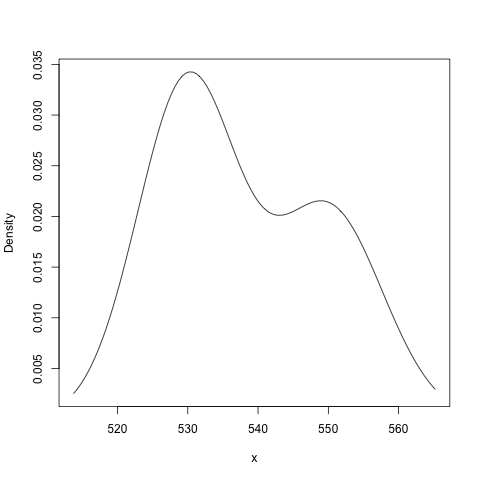
\includegraphics[width=.7\textwidth]{plot_1.png}
        \caption{True model. Mixture of Guassian.}
        \label{Mixture of gaussians}
    \end{subfigure}
    \begin{subfigure}{0.5\textwidth}
        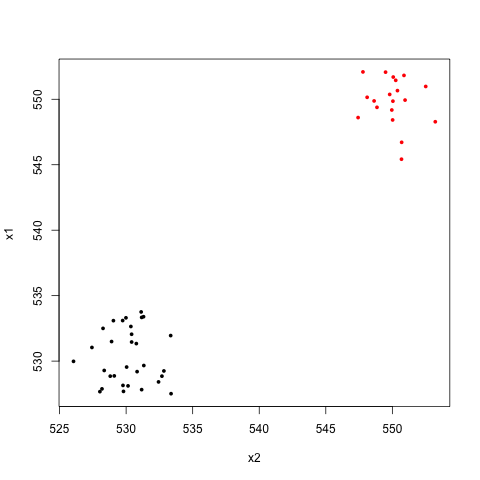
\includegraphics[width=.7\textwidth]{plot_2.png}
        \caption{Sample from the true model}
        \label{Mixture of gaussians}
    \end{subfigure}
\end{figure}


The only information which I would like to consider for prior specification is on the separation of the two mixture weights. Thus I would like to conduct a `non-informative` inference using diffuse prior belief and I would like to avoid any prior ordering of the mean vector. Even if a strong prior belief on the separation of the two mixture weights may help in the simulation procedure, the posterior sample will be spoiled, which will make the inferential estimates ineffective. The label switching problem will be addressed in the next section. 
Prior parameters are the following:
\begin{align*}
& \mu_0 = 0; \ \tau_0 = 1e-6 \\
& a_0 = 1e-3;\  b_0 = 1e-3 \\
& \vec \alpha = (2,2)
\end{align*}

\subsection{Posterior sample}
The Gibbs sampling run for 10.000 iterations, with an initial burn-in of 2.000 samples and thin value of 10. Initial values are $\vec \mu = (500, 600), \vec w = (0.5,0.5)$. 

\begin{figure}[h!]
    \centering
    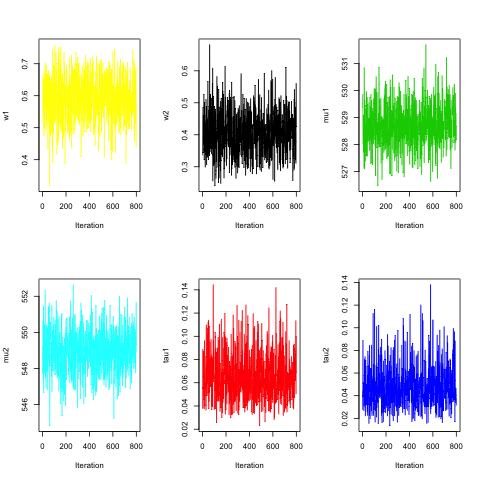
\includegraphics[width=.5\textwidth]{plot_3.png}
    \caption{Traceplot of a single MCMC}
    \label{Monkey measurement}
\end{figure}

In this example we can see the effect of label switching by looking at the trace plot of the the marginal distribution. In fact it seems that the chain starts exploring a subspace which doesn't seem consistent with the rest of the chain. It follows that if we use this sample to make inference, the inference itself will be spoiled by transition between modes. The point estimates are the following:

% latex table generated in R 3.3.2 by xtable 1.8-2 package
% Fri Jul 28 13:22:01 2017
\begin{table}[ht]
\centering
\begin{tabular}{rrrrrrr}
  \hline
 & w1 & w2 & mu1 & mu2 & tau1 & tau2 \\ 
  \hline
Mean & 0.6173 & 0.3827 & 530.8212 & 549.2747 & 0.0698 & 0.0760 \\ 
  Var & 0.0042 & 0.0042 & 0.5366 & 0.8935 & 0.0004 & 0.0008 \\ 
  Tau\_B & 0.0000 & 0.0000 & 0.0063 & 0.0045 & 0.0000 & 0.0000 \\ 
  Gamma\_G & 0.0037 & 0.0037 & 0.5226 & 0.9633 & 0.0004 & 0.0009 \\ 
  T\_eff & 894.5530 & 894.5530 & 800.0000 & 800.0000 & 800.0000 & 777.6688 \\ 
   \hline
\end{tabular}
\end{table}

Notice that the effective sample size is maximum, stating that the parameters of thinning and burn-in helped in reducing the auto correlation between subsequent samples.

\subsection{Label switching}
One interesting aspect of this model is its invariance under permutation, that is the components of the ith units are not identifiable marginally. This aspect can be seen either as a feature or a "bug". It's a feature because for prediction purposes we don't care about the particular ordering of the parameters, while for Bayesian inference we do. As we've seen before, in a C component mixture the number of modes is of the order $O(C!)$, which makes exploration and maximization of the posterior surface obviously harder. This is what is commonly defined as label switching.
In order to solve this problem we can act either on the model, or on a more tailored inferential approach. In the first case, a 'naive' approach is to impose identifiable constraints on the parameter like ordering of the means, which is exactly what we will see in the model proposed in the winbugs example. This approach is not innocuous and leads to at least 3 main shortcomings:
\begin{itemize}
\item  The imposed truncation has no reason to respect the topology of either the prior or the likelihood, in other words we may have high density mode at the margin of the truncated space, which will be disfavored wrt local maxima.
\item It may happen that the posterior sample may heavily modify the prior modeling. 
\item As the number of classes increase, the portion of the space will contain many modes, making identifiabilty difficult.
\end{itemize}
The second approach is to use tailored inferential techniques. In particular we would like to act ex-post, that is after sampling is completed. The idea is to define a suitable pivot point like the MLE or the MAP, and to minimize the $L_{2c}$ norm between the suitable parameter vector and the all its permutation. More formally let $\tau \in \mathcal{T}_c$ be the set of all permutations of $\{1, \cdots, k\}$ we denote by:
\begin{equation}
\tau (\vec \theta, \vec w) = \{ (\theta_{\tau(1)},\cdots, \theta_{\tau(c)}),(\theta_{\w(1)},\cdots, \theta_{\w(c}) \}
\end{equation}

The corresponding permutation of the parameter. Given a sample of size M we do the following:

\begin{enumerate}
\item compute the pivot which is a MC approximation fo the MAP.
\begin{equation}
    (\vec \theta, \vec w)^{i^{\ast}} = \argmax_{i=1, \cdots, M} \pi( (\vec \theta, \vec w)^{(i)} \mid x)
\end{equation}

That is a Monte Carlo approximation of the MAP
\item For each i $\in 1,\cdots, M$ compute:

\begin{equation}
\tau_i = \argmin_{\tau \in \Tau_c} \langle \tau (\vec \theta, \vec w)^{(i)}, \tau (\vec \theta, \vec w)^{(i^{\ast})}\rangle_{2C} 
\end{equation}

\item  Set:
\begin{equation}
(\vec \theta, \vec w)^{(i)} =  \tau(\vec \theta, \vec w)^{(i)}
\end{equation}
\end{enumerate}

Notice that in step 2 we are minimizing a squared distance between two vectors, which resemble a computation of a sequence of loss function for each ith sample that we summarize in the scalar product of the 2k modes. This procedure is well implemented in R, in the ```label.switching``` package. Suitable initialization points to use as pivot points are the MLE estimates of the parameters that can be obtained via the ```MCclust``` package that use the EM algorithm to find the maximum likelihood estimate. With this in mind we can initialize the chain and compare the results with the previous run:

% latex table generated in R 3.3.2 by xtable 1.8-2 package
% Fri Jul 28 13:24:24 2017
\begin{table}[ht]
\centering
\begin{tabular}{rrrrrrr}
  \hline
 & w1 & w2 & mu1 & mu2 & tau1 & tau2 \\ 
  \hline
Mean & 0.3842 & 0.6158 & 548.3712 & 531.7029 & 0.0763 & 0.0694 \\ 
  Var & 0.0036 & 0.0036 & 15.4946 & 15.6496 & 0.0007 & 0.0004 \\ 
  Tau\_B & 0.0000 & 0.0000 & 0.1605 & 0.1223 & 0.0000 & 0.0000 \\ 
  Gamma\_G & 0.0039 & 0.0039 & 19.0515 & 17.3069 & 0.0008 & 0.0004 \\ 
  T\_eff & 800.0000 & 800.0000 & 800.0000 & 800.0000 & 800.0000 & 800.0000 \\ 
   \hline
\end{tabular}
\end{table}

We note that the effect of label switching on the previous to the relabeling procedure, completely mess the order of the true proportion for the simulation. After relabeling, even if we don't have significant changes in point estimates, the effective sample size drastically increase, resulting in a more robust inference for the variance of each parameter.

\begin{figure}[h!]
    \centering
    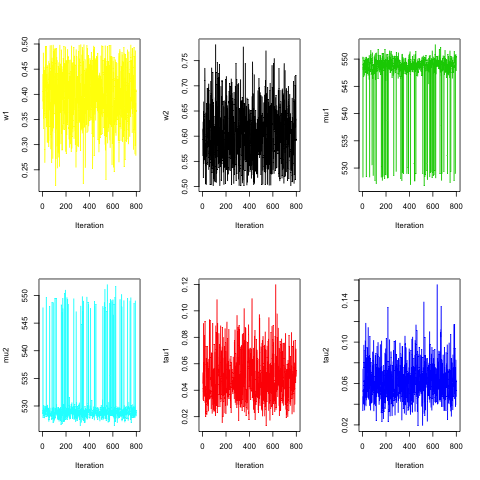
\includegraphics[width=.5\textwidth]{plot_4.png}
    \caption{Traceplot after label switching}
    \label{Monkey measurement}
\end{figure}

\section{Experiment}
In the following section we are going to evaluate the following inference procedure to obtain a 'clean' sample from the posterior distribution.
\begin{enumerate}
\item Compute MLE estimates for the parameter vector
\item Obtain a posterior sample from the GIBBS sampler
\item Use the Pivotal Reordering Algorithm (PRA) ex-post
\end{enumerate}
Then we will compute point estimates, DIC and predictive check to discuss and evaluate the model proposed by Robert et al (1998) which is the standard implementation in Winbugs. An interesting aspect about this second model is that it uses a single precision parameter $\tau$ and it imposes an order of the mean by shifting the mean of the second class with positive noise.

While in our case we relax the assumption of single variance for the same mean vector because we may want to account delays between measurements or reaction time of different pigment. We can use the BIC criterion provided by the `MC clust package` to check if the burden of an extra parameter it is not too expensive. In fact in the following table we can see that the difference between the two models is small enough to justify its uses.

\begin{table}[ht]
\centering
\begin{tabular}{rrr}
  \hline
 BIC & \vec \mu & \vec \sigma^2 \\ 
  \hline
    1 & -330.06 & -330.06 \\ 
  2 & -324.92 & -323.56 \\ 
  3 & -329.06 & -331.75 \\ 
   \hline
\end{tabular}
\end{table}

\subsection{Data}
The dataset is made of 48 measurements coming from a single female squirrel monkey. The measurements have been obtained for individual photo receptors that had been shown behaviourally to be trichromatic, that is to have developed 3 different channels to convey visual information to the brain.  The first analysis coming from Bowmaker et al. (1985) use MLE to evaluate the best model as a composition of three underlying distribution. It follows a general description of the data, and the histogram.

\begin{figure}[h!]
    \centering
    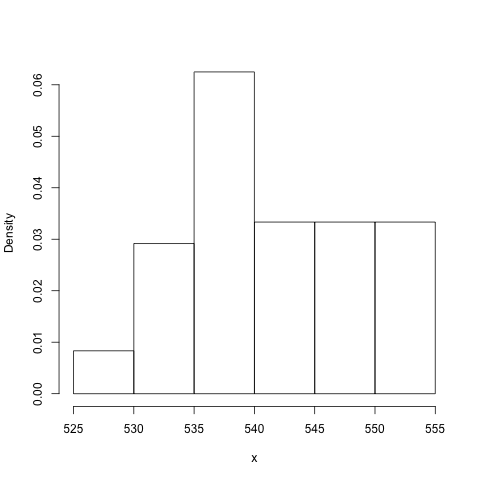
\includegraphics[width=.4\textwidth]{plot_5.png}
    \caption{Histogram of measurements}
    \label{Monkey measurement}
\end{figure}

\begin{table}[ht]
\centering
\begin{tabular}{rrrrrrr}
  \hline
 & Min. & 1st Qu. & Median & Mean & 3rd Qu. & Max. \\ 
  \hline
 & 529.00 & 536.10 & 540.00 & 541.50 & 548.80 & 553.20 \\ 
   \hline
\end{tabular}
\end{table}


\section{Proposed model}
Monkeys have been tested for red and green lights for which the normalized spectra ranges between 400 to 700 for the red light and from 400 to 630 for the green one, with pick around 550. Considering this prior information we may want to set the initial values for $\mu_1, \mu_2$ to be in this range, respectively 500, and 600. The mixture weights will be initialized equal, namely $w_1, w_2 = 0.5$.
We can generate the first run of the Gibbs sampling with 10.000 samples, with thin of 20 and burnin of 2000. Before looking at the actual point estimates, let's pause on the traceplot.

\subsection{Spoiled sample}
The trace plot (fig. 5) shows that the sampler explored different portion of the parameter space, under the same "label" this can be spotted by noticing the `unusual` jumps in the trace. It seems that $\vec \mu \ and \  \vec w$ suffer the most of this behavior. One interesting and reasonable consequence of this exploration behavior is that different parameters may end up having high auto-correlation even in with large lag windows. As a result if we would accept posterior point estimates and intervals, we would expect similar values for different parameters, but more important an underestimate of the sample variance estimate. 

\subsection{Ex-post relabelling}
The application of the PRA requires a pivot point for each parameter. For this purpose we can use the `McClust` package to find the MLE estimates via the EM algorithm and use it as starting points for the new chain and pivot points for the re-labelling algorithm. Looking at the estimated densities we notice that there are traces of the mixing labels but it's much lower. As a positive side effect, we should also get lower auto correlation between components of the parameter vector.

\begin{figure}[h!]
    \begin{subfigure}{0.5\textwidth}
        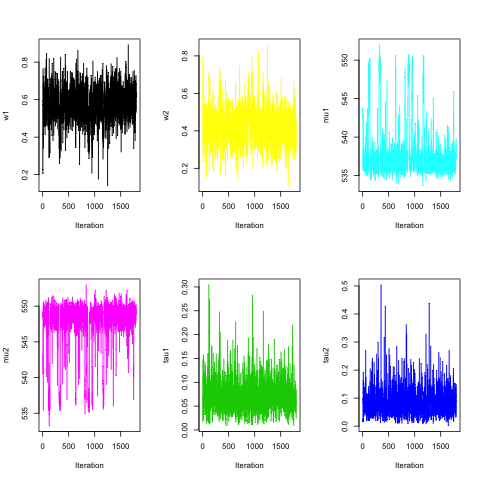
\includegraphics[width=.4\textwidth]{plot_6.png}
        \caption{Traceplot of the first run.}
        \label{Monkey measurement}
    \end{subfigure}
    \begin{subfigure}{0.5\textwidth}
        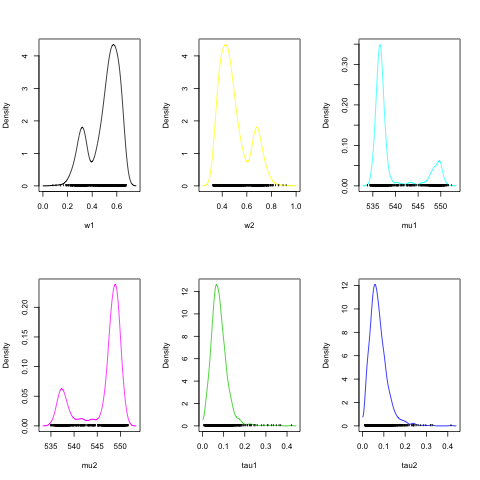
\includegraphics[width=.4\textwidth]{plot_7.png}
        \caption{Marginal densities post PRA}
        \label{Monkey measurement}
    \end{subfigure}
\end{figure}

\subsection{Point estimate}
The following table is split in two sections. The first section shows point estimates with the spoiled sample and the second shows the effect of the relabelling procedure.
For each run I estimated mean, sample variance, batch variance,the initial sequence estimator and the effective sample size. Interestingly enough the two variance estimators can detect the label switching problem and one explanation could be that both of them compute partial estimates on sub sample of the overall chain which will likely contain samples coming from different components of the same parameter vector.

\begin{table}[ht]
\centering
\begin{tabular}{rrrrrrr}
  \hline
 sec. I & w_1 & w_2 & \mu_1 & \mu_2 & \tau_1 & \tau_2 \\ 
  \hline
    \hat{\mu} & 0.5752 & 0.4248 & 537.8392 & 547.5201 & 0.0708 & 0.0816 \\ 
  \hat{\sigma}^2  & 0.0092 & 0.0092 & 11.0087 & 12.8970 & 0.0012 & 0.0024 \\ 
  \hat{\tau}_B^2 & 0.0014 & 0.0014 & 6.6756 & 6.7660 & 0.0001 & 0.0001 \\ 
  \hat{\gamma}_G^2 & & 0.0459 & 0.0459 & 203.3975 & 214.8883 & 0.0017 & 0.0031 \\ 
  \hat{\tau}_{eff} & 430.3858 & 430.3858 & 82.1076 & 107.5008 & 1451.3522 & 1486.9215 \\ 
   \hline
   sec. II &\\
    \hline
  \hat{\mu}  & 0.5041 & 0.4959 & 539.0434 & 546.3235 & 0.0791 & 0.0746 \\ 
  \hat{\sigma}^2  & 0.0142 & 0.0142 & 23.7958 & 20.7495 & 0.0016 & 0.0018 \\ 
  \hat{\tau}_B^2  & 0.0005 & 0.0005 & 0.7997 & 0.8483 & 0.0000 & 0.0001 \\ 
  \hat{\gamma}_G^2  & 0.0176 & 0.0176 & 25.9539 & 24.6188 & 0.0020 & 0.0024 \\ 
  \hat{\tau}_{eff} & 1559.5617 & 1559.5617 & 1800.0000 & 1659.7700 & 1523.0408 & 1589.1159 \\ 
\end{tabular}
\end{table}

\subsection{Model selection}
To complete the analysis, we can look at the capability of the model to replicate the observed data, and the DIC. The ability to replicate the data can be easily done by sampling a single value from a mixture of Gaussian, for each posterior sample. 

\begin{figure}[h!]
    \centering
    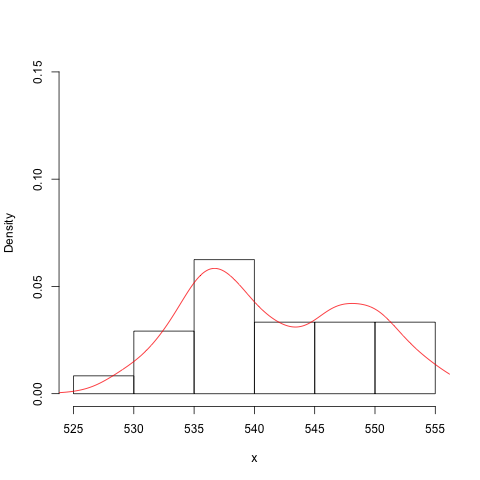
\includegraphics[width=.3\textwidth]{plot_8.png}
    \caption{Posterior predictive check}
    \label{Monkey measurement}
\end{figure}

The DIC for the model is 310.6009.

\section{JAGS model}
The prior model specification in the JAGS example are the following:
\begin{align*}
\tau &\sim \mathcal{G}(0.01, 0.01) \\
\epsilon &\sim \mathcal{N}(0, 1e^{-3}) \mathbb{I}_{(0, \infty)}(\epsilon) \\ 
\mu_1 &\sim \mathcal{N}(0, 1e^{-3}) \\
\mu_2 &= \mu_1 + \epsilon \\
\vec w &\sim \mathcal{D}(1, \vec \alpha)
\end{align*}

\subsection{Simulation}
In this model we have the same diffuse prior specification except for the fact that $\mu_2$ is shifted from $\mu_1$ with some positive random noise, which imply the separation and ordering of the mean vector. The initial value for the chain are the following $\mu_1 = 535, \ \theta = 5, \ \tau = 0.1,\ (w_1, w_2) = 0.5$. We run the chain for 20.000 iterations, with an initial burn-in of 2.000, and thin of 10. Looking at fig 9, the traceplot for $\mu_1, \mu_2$ doesn't show the same irregularities that we observed in the previous model and that's a natural consequence of the sequential order imposed in the prior specification. 

\begin{figure}[h!]
    \centering
    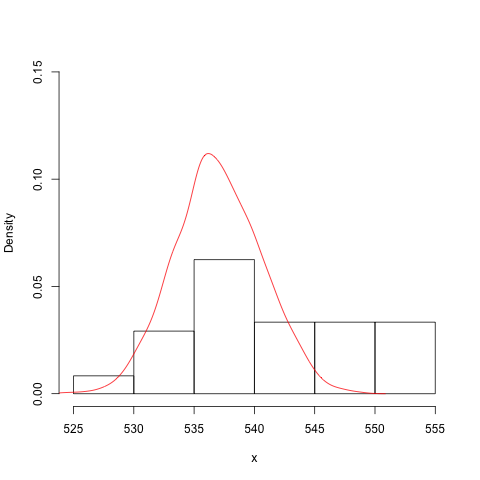
\includegraphics[width=.3\textwidth]{plot_10.png}
    \caption{Traceplot JAGS model}
    \label{Monkey measurement}
\end{figure}

\subsection{Point estimate}
The results of the posterior estimates are the following. We notice that this model produce samples with much lower variance that there is relevant difference in the estimates for the mixture weight. This is reasonable if we consider that we imposed a "blind" separation and order in the parameter space.

% latex table generated in R 3.3.2 by xtable 1.8-2 package
% Fri Jul 28 13:32:37 2017
\begin{table}[ht]
\centering
\begin{tabular}{rrrrrrr}
  \hline
 & w1 & w2 & mu1 & mu2 & tau & x\_new \\ 
  \hline
Mean & 0.5952 & 0.4048 & 536.7747 & 548.7103 & 0.0733 & 536.9903 \\ 
  Var & 0.0112 & 0.0112 & 1.1953 & 2.3868 & 0.0005 & 13.1606 \\ 
  Tau\_B & 0.0003 & 0.0003 & 0.0264 & 0.0544 & 0.0000 & 0.3175 \\ 
  Gamma\_G & 0.0114 & 0.0114 & 1.3528 & 2.5043 & 0.0005 & 13.5918 \\ 
  T\_eff & 1800.0000 & 1800.0000 & 1711.7000 & 1800.0000 & 1800.0000 & 1800.0000 \\ 
   \hline
\end{tabular}
\end{table}

\subsection{Model selection}
As for the previous model, we now turn computing the posterior predictive distribution and the DIC. As we can see from fig XXX, this model doesn't seem to be able to reproduce new samples along the overall spectra of possible measurements. An hypothesis for this effect it may rely on the difference in mixture weights estimates. Finally the DIC for this model is 362.3982.

\begin{figure}[h!]
    \centering
    \includegraphics[width=.3\textwidth]{plot_11.png}
    \caption{Posterior predictive check}
    \label{Monkey measurement}
\end{figure}

\section{Results and discussion}
As a short summary, We reviewed the basics of finite mixture of normal model, providing the mixture weights and completion representations. We dived into the inference problem connected to the in variance property of the likelihood, and more generally the presence of multiple modes. In the inferential setup, this problem is also know as label switching and we reviewed the two core ideas to clean a spoiled sample, namely prior ordering and ex-post relabelling. Then we defined the full Bayesian model using conjugate priors and separated variances, one for each mixture component. Finally we reviewed the model suggest by JAGS and we discussed the relevant differences, noticing that the provide model is less powerful in generating new data.

The code can be found \href{https://github.com/d3sm0/mixgauss}{here}.

\section{References}
\begin{reference}
    \bibitem{Grayer} Charles Grayer {\em Practical Markov Chain Monte Carlo} 
    1995: Statistical Science, Vol. 7, No. 4.
    \bibitem{Robert} Jean-Michel Marin, Kerrie Mengersen and Christian P. Robert {\em
    Bayesian Modelling and Inference on Mixtures of Distributions}
    \bibitem{Bowmaker} J.K. Bowmajer, G.H. Jacobs, J. Spiegelhalter and J.D. Mollon{\em
    Two types of trichromatic squirrel monkey share a pigment in the red-green spectral region}
    1985
\end{reference}

\end{document}